
\chapter{Introduction}
%\addcontentsline{toc}{chapter}{Introduction}


\minitoc

One fundamental goal of Artificial Intelligence (\ai) is to design embodied autonomous interactive agents that can evolve in various environments and complete a wide range of tasks. To that end, researchers in \ai take several angles of attack and rely on different paradigms that consider different drivers for learning. In Reinforcement Learning (\rl)~\citep{sutton2018reinforcement}, agents learn from \textit{exploration} of their environment. They rely solely on their experience of the world in order to solve a pre-defined task. In Imitation Learning (\il)~\citep{pomerleau1991efficient}, agents learn from \textit{demonstrations}, i.e. trajectories provided by an expert that correspond to the transitions required to take to solve a pre-defined task.  In Multi-Agent Learning~\citep{LITTMAN1994157}, agents learn in \textit{cooperation} and need to interact with each other in order to solve collaborative tasks.


Recent extensions of \rl algorithm have shown success in solving a wealth of problems such as playing the Atari videogames at super-human levels~\citep{mnih2015human}, beating chess and go world champions~\citep{silver2016mastering}, controlling stratospheric baloons~\citep{bellemare2020autonomous} or even maintaining plasma in fusion reactors~\citep{degrave2022magnetic}. Similarly, \il methods coupled to Transformers~\citep{vaswani2017attention} have enabled the training of a generalist agent on a massive dataset of diverse interactions~\citep{reed2022a}. It has also been used to perform in-context reinforcement learning via algorithm distillation~\citep{laskin2022incontext}. Finally, multi-agent methods have permitted populations of agents to play hide and seek~\citep{Baker2020Emergent} or even to collaboratively solve common-pool resource problems~\citep{perolat2017commonpool}.

But unlike humans, these algorithms are still heavily sample-inefficient, requiring billions of transitions to become proficient on isolated tasks. Most importantly, they lack the ability to generalize and transfer across a wide variety of problems, to be creative, and tackle tasks never seen during training. They are far from displaying human-like capabilities in terms of open-ended learning. This is, perhaps, because they rely on isolated signals for learning. The way forward might be to build on child development theory and to consider learning from \textit{sociocultural interactions}. Indeed humans are social beings, they interact and cooperate with their peers~\citep{tomasello_cultural_1999,tomasello_understanding_2005, brewer2014addressing}. As soon as they discover and learn a language, they assimilate thousands of years of experience embedded in their culture~\citep{bruner1991narrative}.  Most of their skills could not be learned in isolation. Formal education teaches them to reason systematically, books teach them history, and YouTube might teach them how to cook. Most importantly, humans' values, traditions, norms, and most of their goals are cultural in essence.

The present research proposes to immerse artificial agents in social contexts in order to observe the impact of sociocultural interactions on learning. As displayed in figure~\ref{fig:intro_chapter_def}, it has a dual objective. In the first part of this manuscript, we propose to use artificial agents as an anthropological tool to study the formation of cultural conventions in populations of individuals. More specifically, we investigate the key mechanisms required for the self-organization of cultural models between artificial agents in absence of pre-existing conventions. In the second part, we focus on autonomous artificial agents exploiting already existing cultural conventions to augment their capabilities in the open-ended skill acquisition problem. To accomplish this, we build on previous theories at the intersection of developmental psychology and machine learning to introduce a new framework coined \textit{Vygotskian Artificial Intelligence} which enables sociocultural interactions to transform agents' learning signal, yielding better learners. 

%
\begin{figure}[!h]
\centering
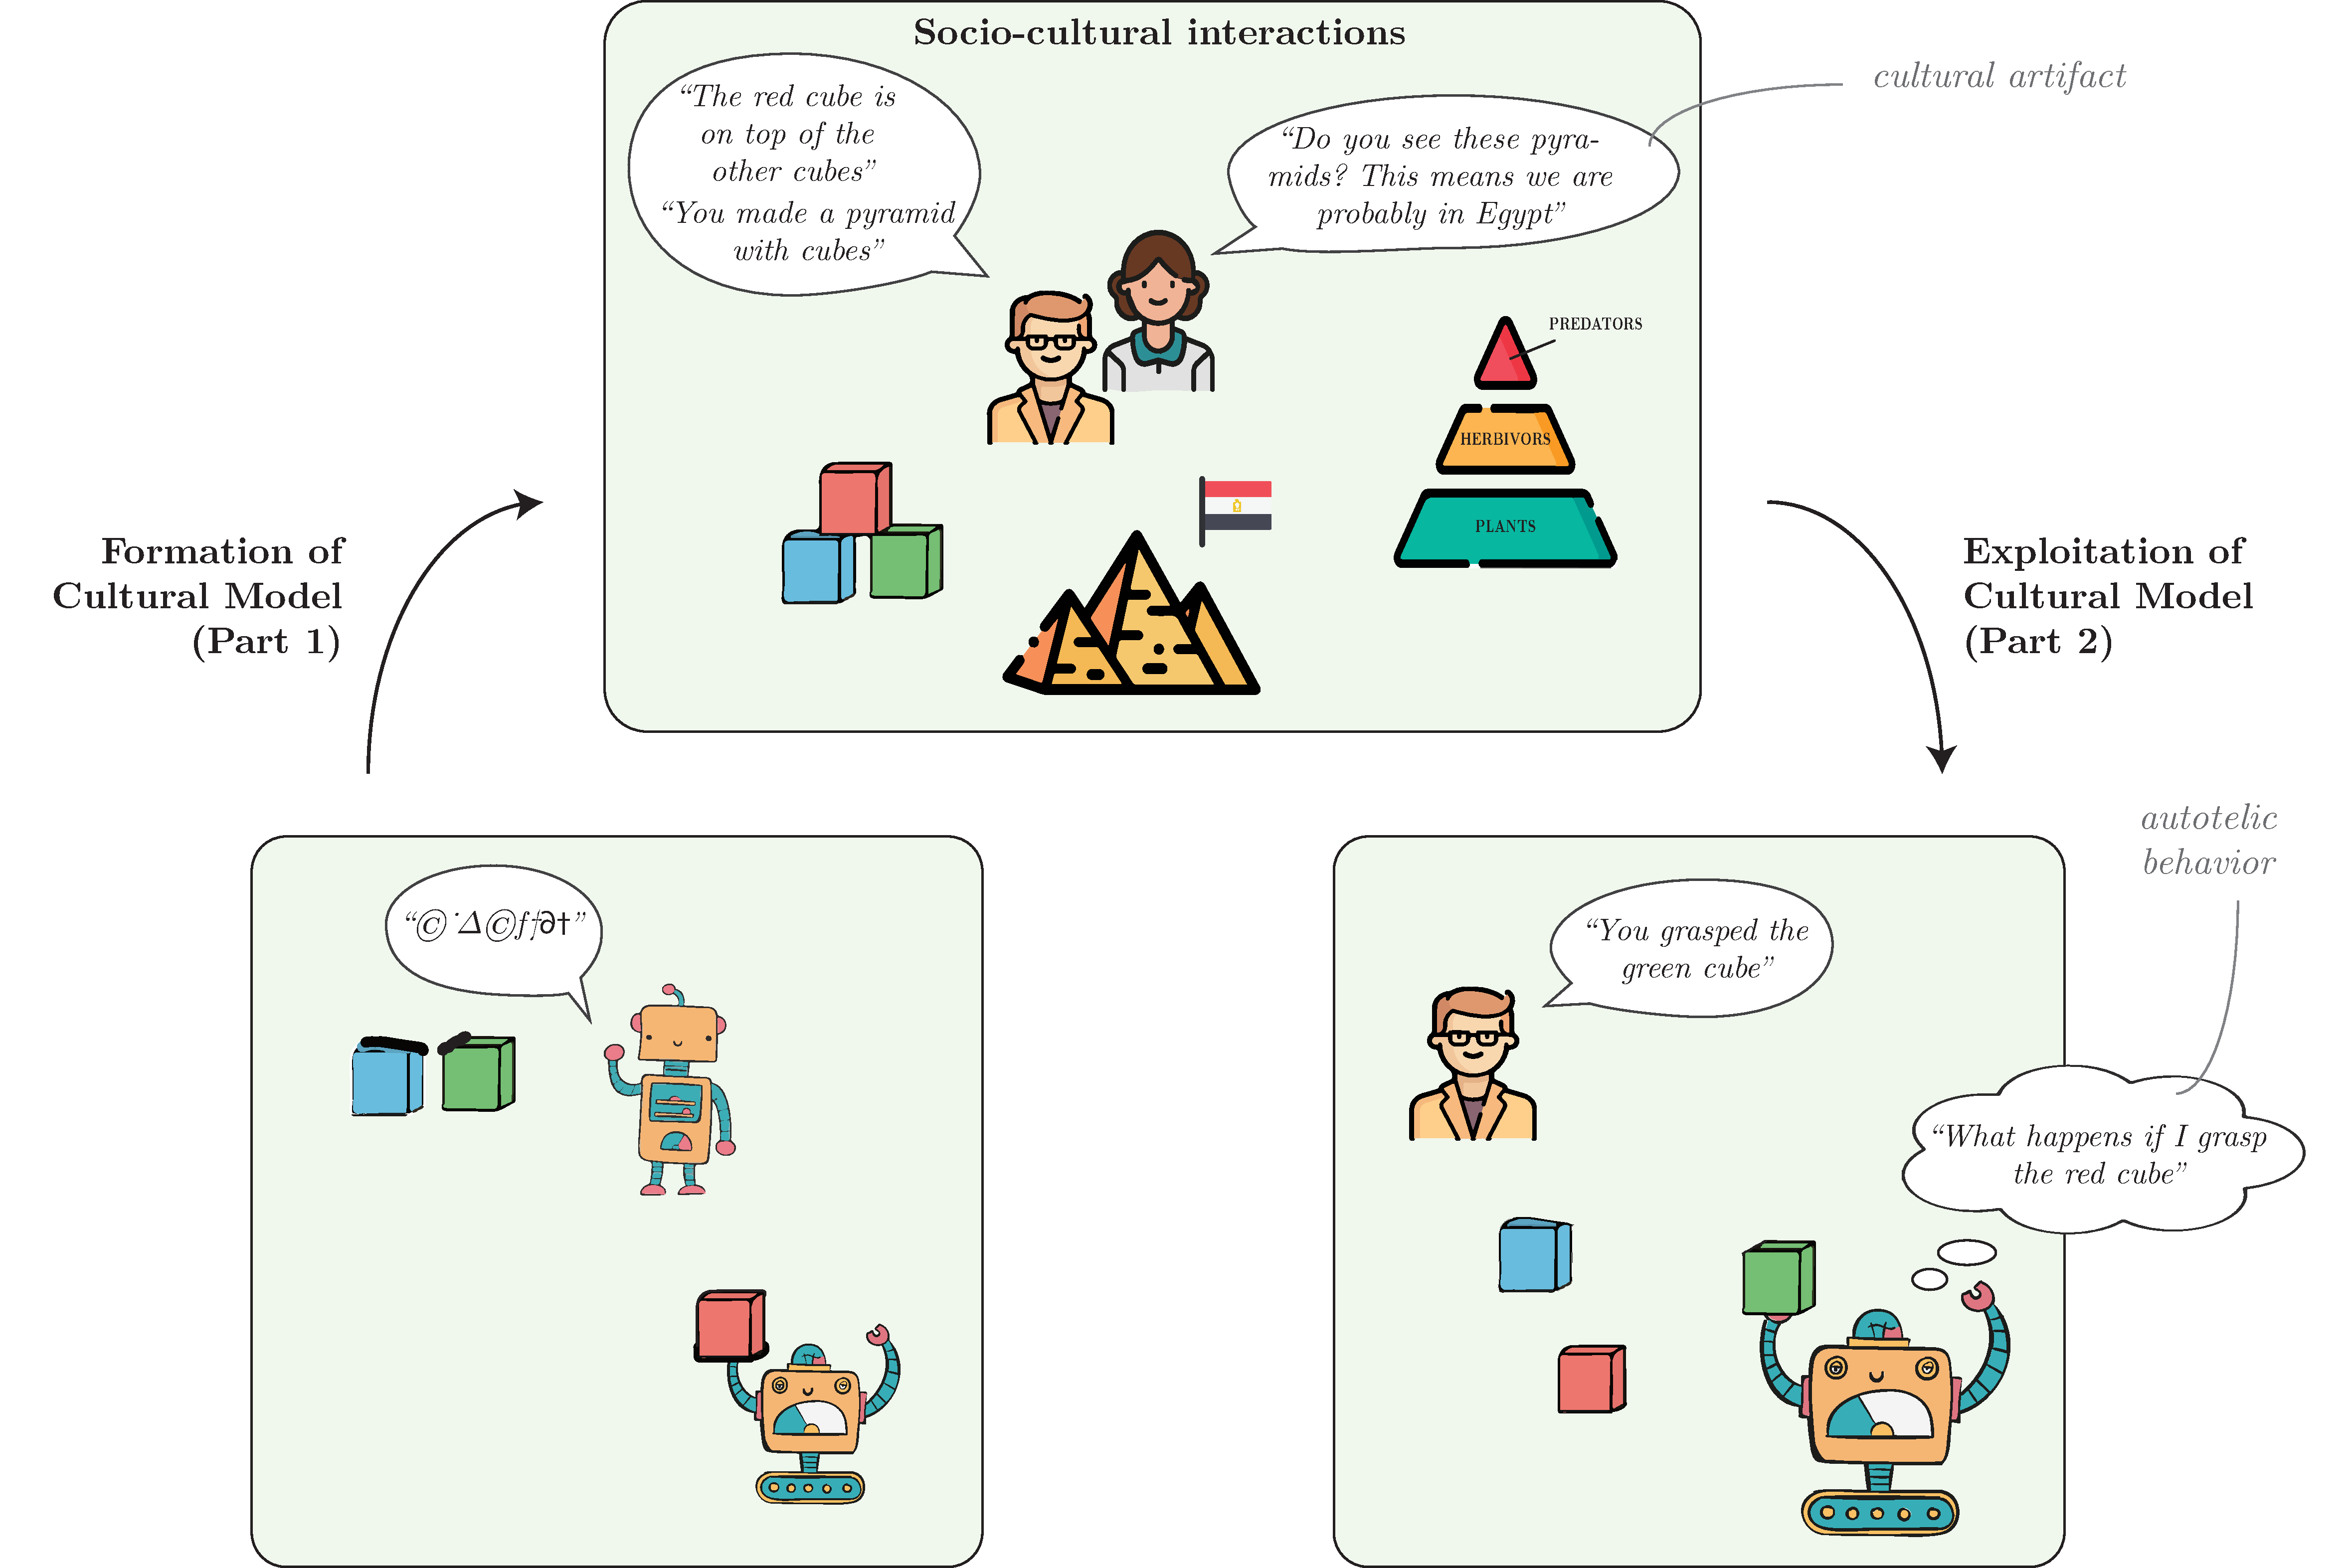
\includegraphics[width=1\textwidth]{intro/intro_chapter_def.pdf}
\caption{\textbf{Dual organization of the present research.} [...]}
\label{fig:intro_chapter_def}
\end{figure}

The remaining of this introduction presents key features of human learning that enable us to define the important notions of "autotelic learning" and "cultural convention" at the center of this research. We then 	


\section{Humans are goal-directed social learners}

Humans are an incredible source of inspiration for \ai. They are the fastest learning system we can ever witness. Within only a few years, children learn to crawl and navigate their home, to identify and manipulate objects, they even learn to speak and interact with their peers. How do they reach such a level of proficiency in such a short period of time? 

\paragraph{Humans are autotelic learners}

A central aspect of human development is the notion of goal. \citet{elliot2008goal} propose the following goal construct definition:
\begin{quote}
    \textit{A goal is a cognitive representation of a future object that the organism is committed to approach or
    avoid}~\citep{elliot2008goal}.
\end{quote}


intrinsic motivation (Piaget?)

In particular, children's exploration seems to be driven by intrinsically motivated brain processes that trigger spontaneous exploration for the mere purpose of experiencing novelty, surprise or learning progress~\citep{gopnik1999scientist,kaplan2007search,kidd_psychology_2015}. During exploratory play, children can also invent and pursue their own problems [19].

\citet{csikzentmihalyi1997finding} uses the term autotelic in his theory of flow to describe those agents or activities that are intrinsically motivated. 

Steels will later use the term to designate [insert quote from steel]

\begin{tcolorbox}
\small
\paragraph{Definition}
\gls{Autotelic}: from the Greek \textit{auto} (self) and \textit{telos} (end, goal), characterizes agents that generate their own goals and learning signals. In is equivalent to \textit{intrinsically motivated and goal-conditioned}.
\end{tcolorbox}

\paragraph{Humans are social learners}

Humans are social beings; intrinsically motivated to interact and cooperate with their peers~\citep{tomasello_cultural_1999,tomasello_understanding_2005, brewer2014addressing}. 

This knowledge, and some argue, some of our highest cognitive functions such as abstraction, compositional imagination, or relational thinking, are formed through linguistic and cultural interactions with others

 For Vygotsky, linguistic social interactions such as descriptions, explanations, corrections, or play start as interpersonal processes before they are turned into intrapersonal cognitive processes through the process of internalization. 33–35 Following his vision, many psychologists,36–38 linguists,39–41, and philosophers42–45 argued for the importance of socio-cultural interactions in the development of human intelligence.

\begin{tcolorbox}
\small
\paragraph{Definition}
\gls{Cultural Model}: element of language or social interaction from which meaning can be derived.
\end{tcolorbox} 


\section*{Towards Interactive Social Autonomous Agents}

Drawing inspiration from children 

Not necessarily a shift of paradigm but rather using social interactions (language and culture rachets) inside previous paradigms:

\begin{figure}[!h]
\centering
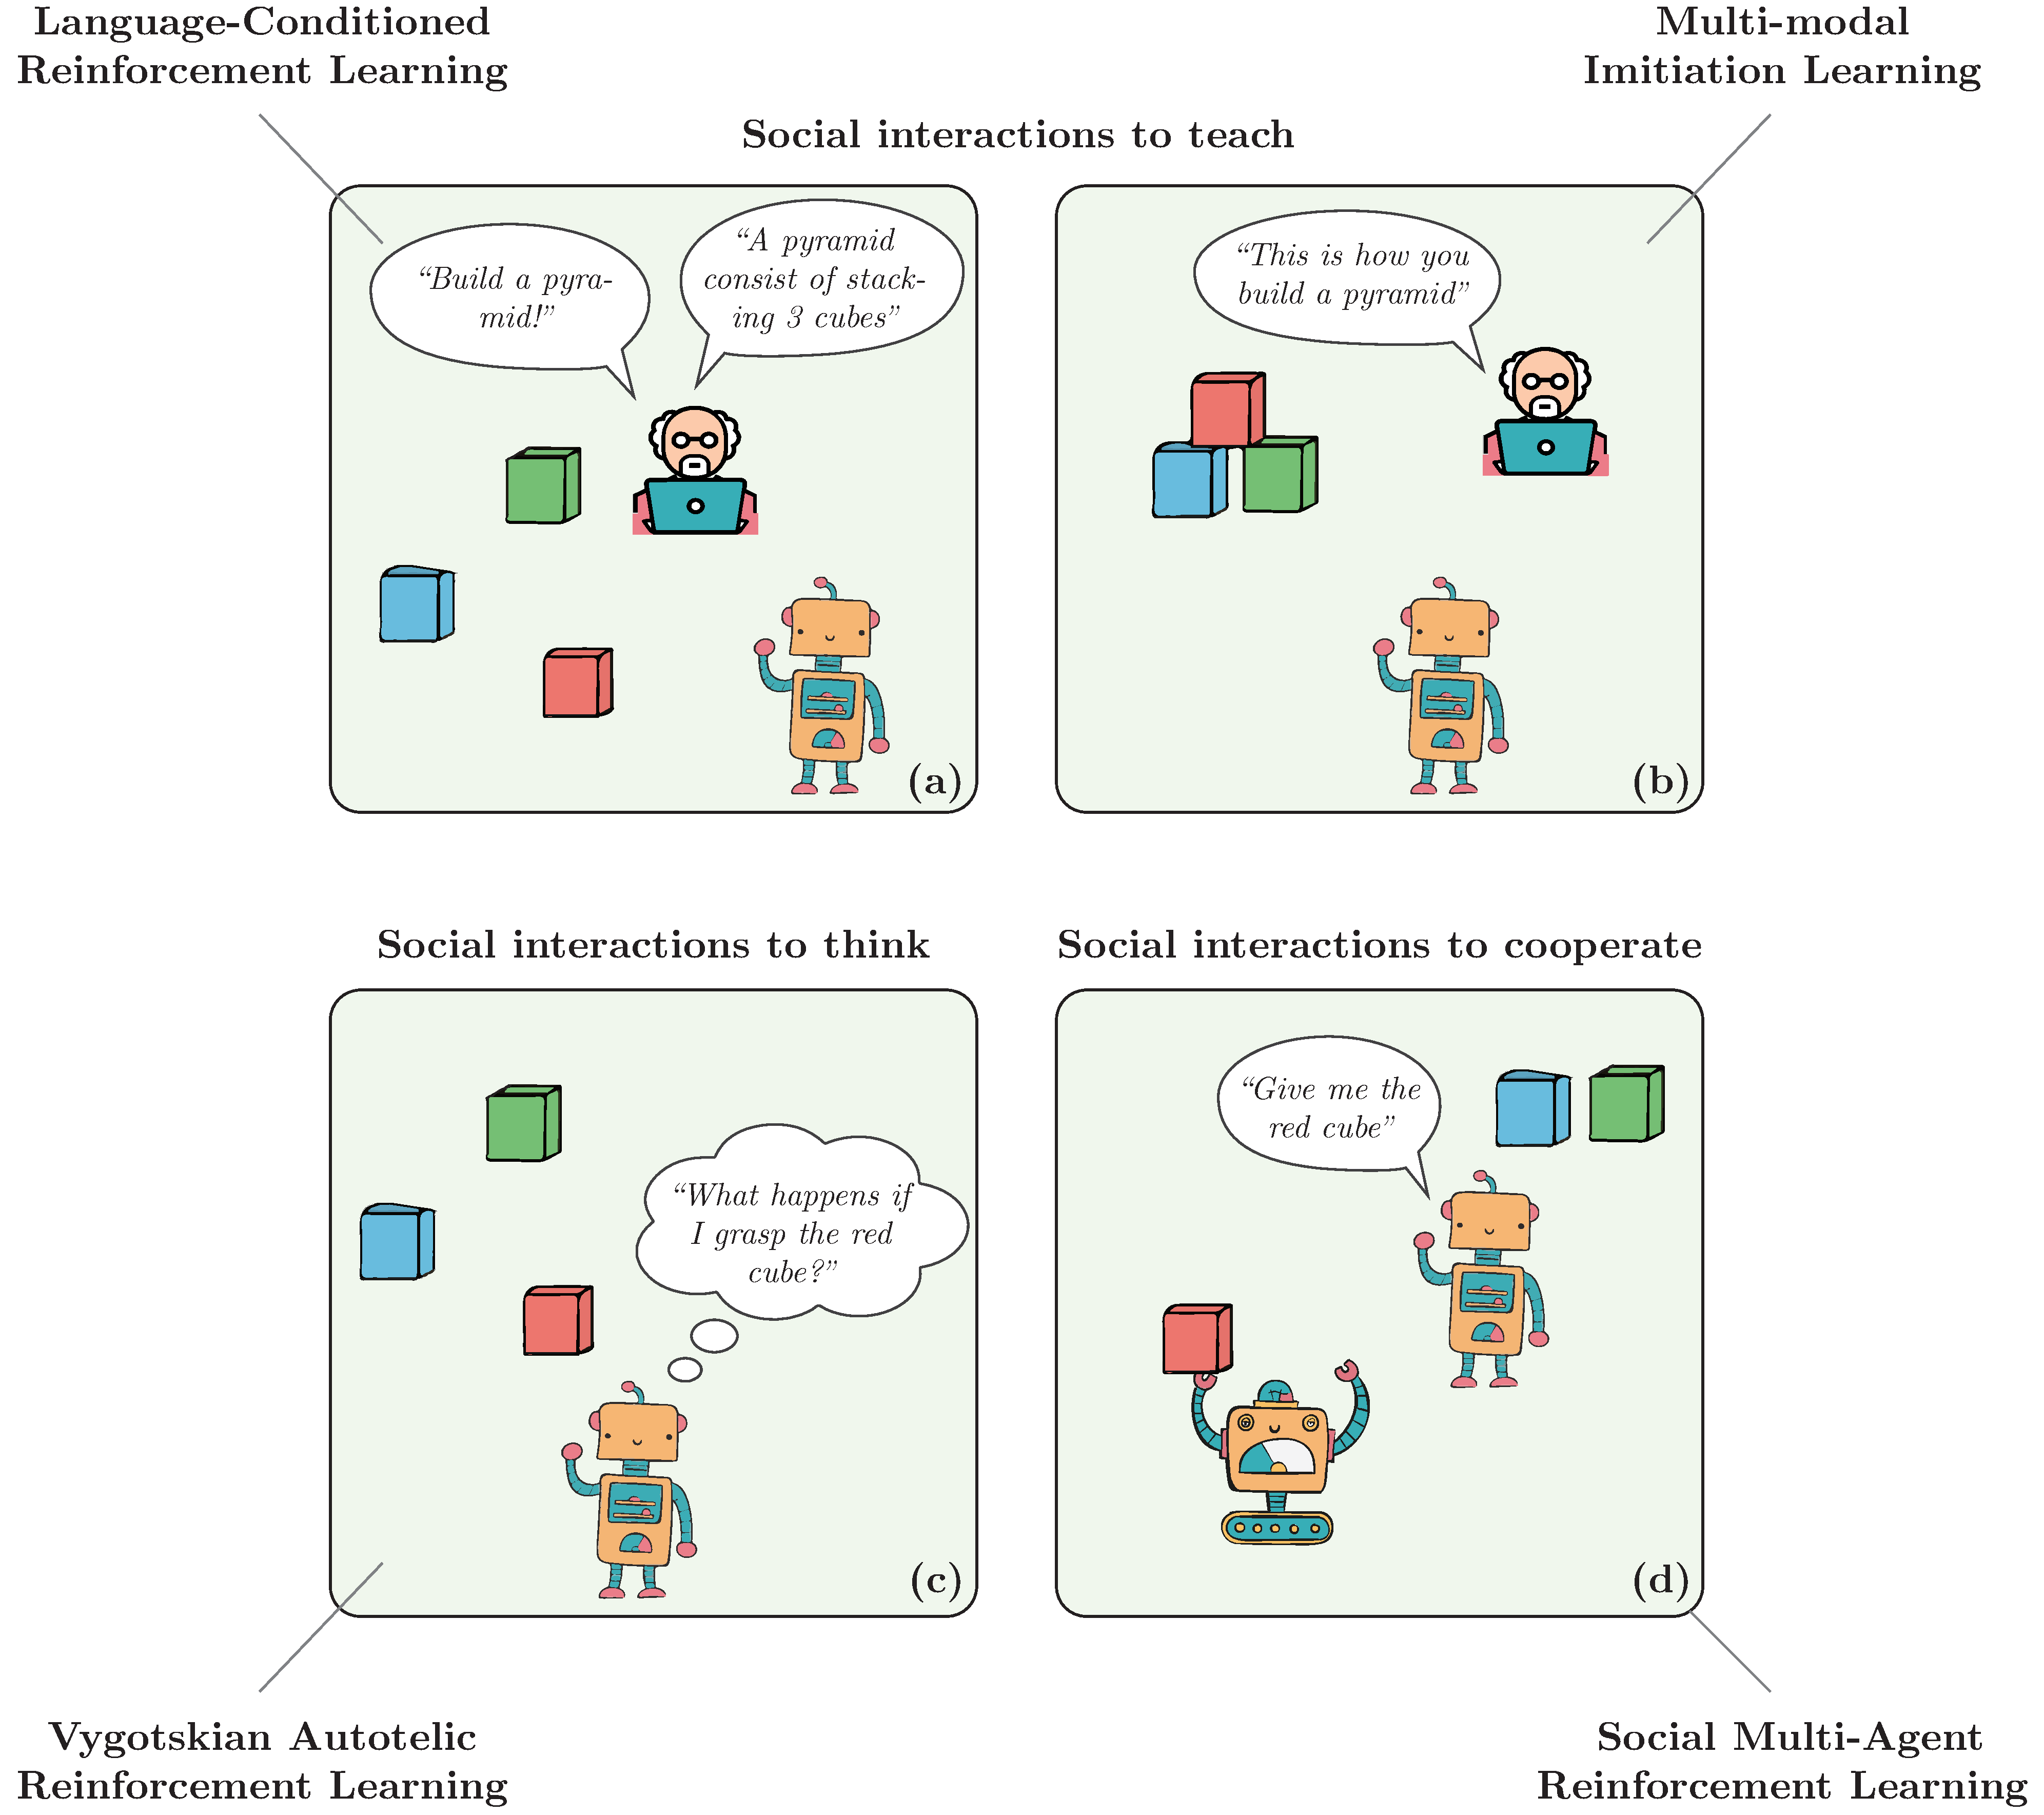
\includegraphics[width=1\textwidth]{intro/language_paradigms.pdf}
\caption{}
\label{fig:intro_language_paradimgs}
\end{figure}

Inside social interaction is language and culture rachets they can be used to:
\begin{itemize}[noitemsep]
\item Language to cooperate 
\item Language to teach \cite{sigaud2021towards}
\item Language to organize thoughts	
\end{itemize}


\paragraph{Objectives and Contributions}

The end goal of the present research is to make progress towards the autonomous acquisition of repertoires of skills. 

We advocate for socio-cultural interactions as the driver of learning as such the 


This manuscript is organized around two main questions:
%
\begin{enumerate}[noitemsep]
	\item How can such a cultural model emerge in populations of agents?
	\item How can agents leverage existing cultural models to become better learners? 
\end{enumerate}

There is no open-endedness without culture. From an engineering perspective, building open-ended environments for artificial agents requires a community effort.

Culture as youtube videos (from perspective)

Citation (bruner, vygotsky)

\clearpage

\paragraph{Chronological order of publications}

\paragraph{Collaborations}



